\section{Results}
\label{sec:results}

Our first set of experiments investigates the relative responses of the log-loss and Brier metrics as a function of isolated systematic effects imposed on baselines of the best possible classifier.

\subsection{Mock classifier systematics}
\label{sec:mockresults}

Figure~\ref{fig:cruise} shows the effect of adding each of four forms of error to a perfect classification, one class at a time, and calculating the metrics with flat weightings.
We confirm that more palatable effects affect the metric values in minor ways and those considered most severe have a more obvious effect.
Both metrics are appropriate for singling out a classifier that enables any class to subsume other classes, thereby confirming that the cruise control classifier will not in general outscore a classifier that avoids subsuming.

\begin{figure}
	\begin{center}
		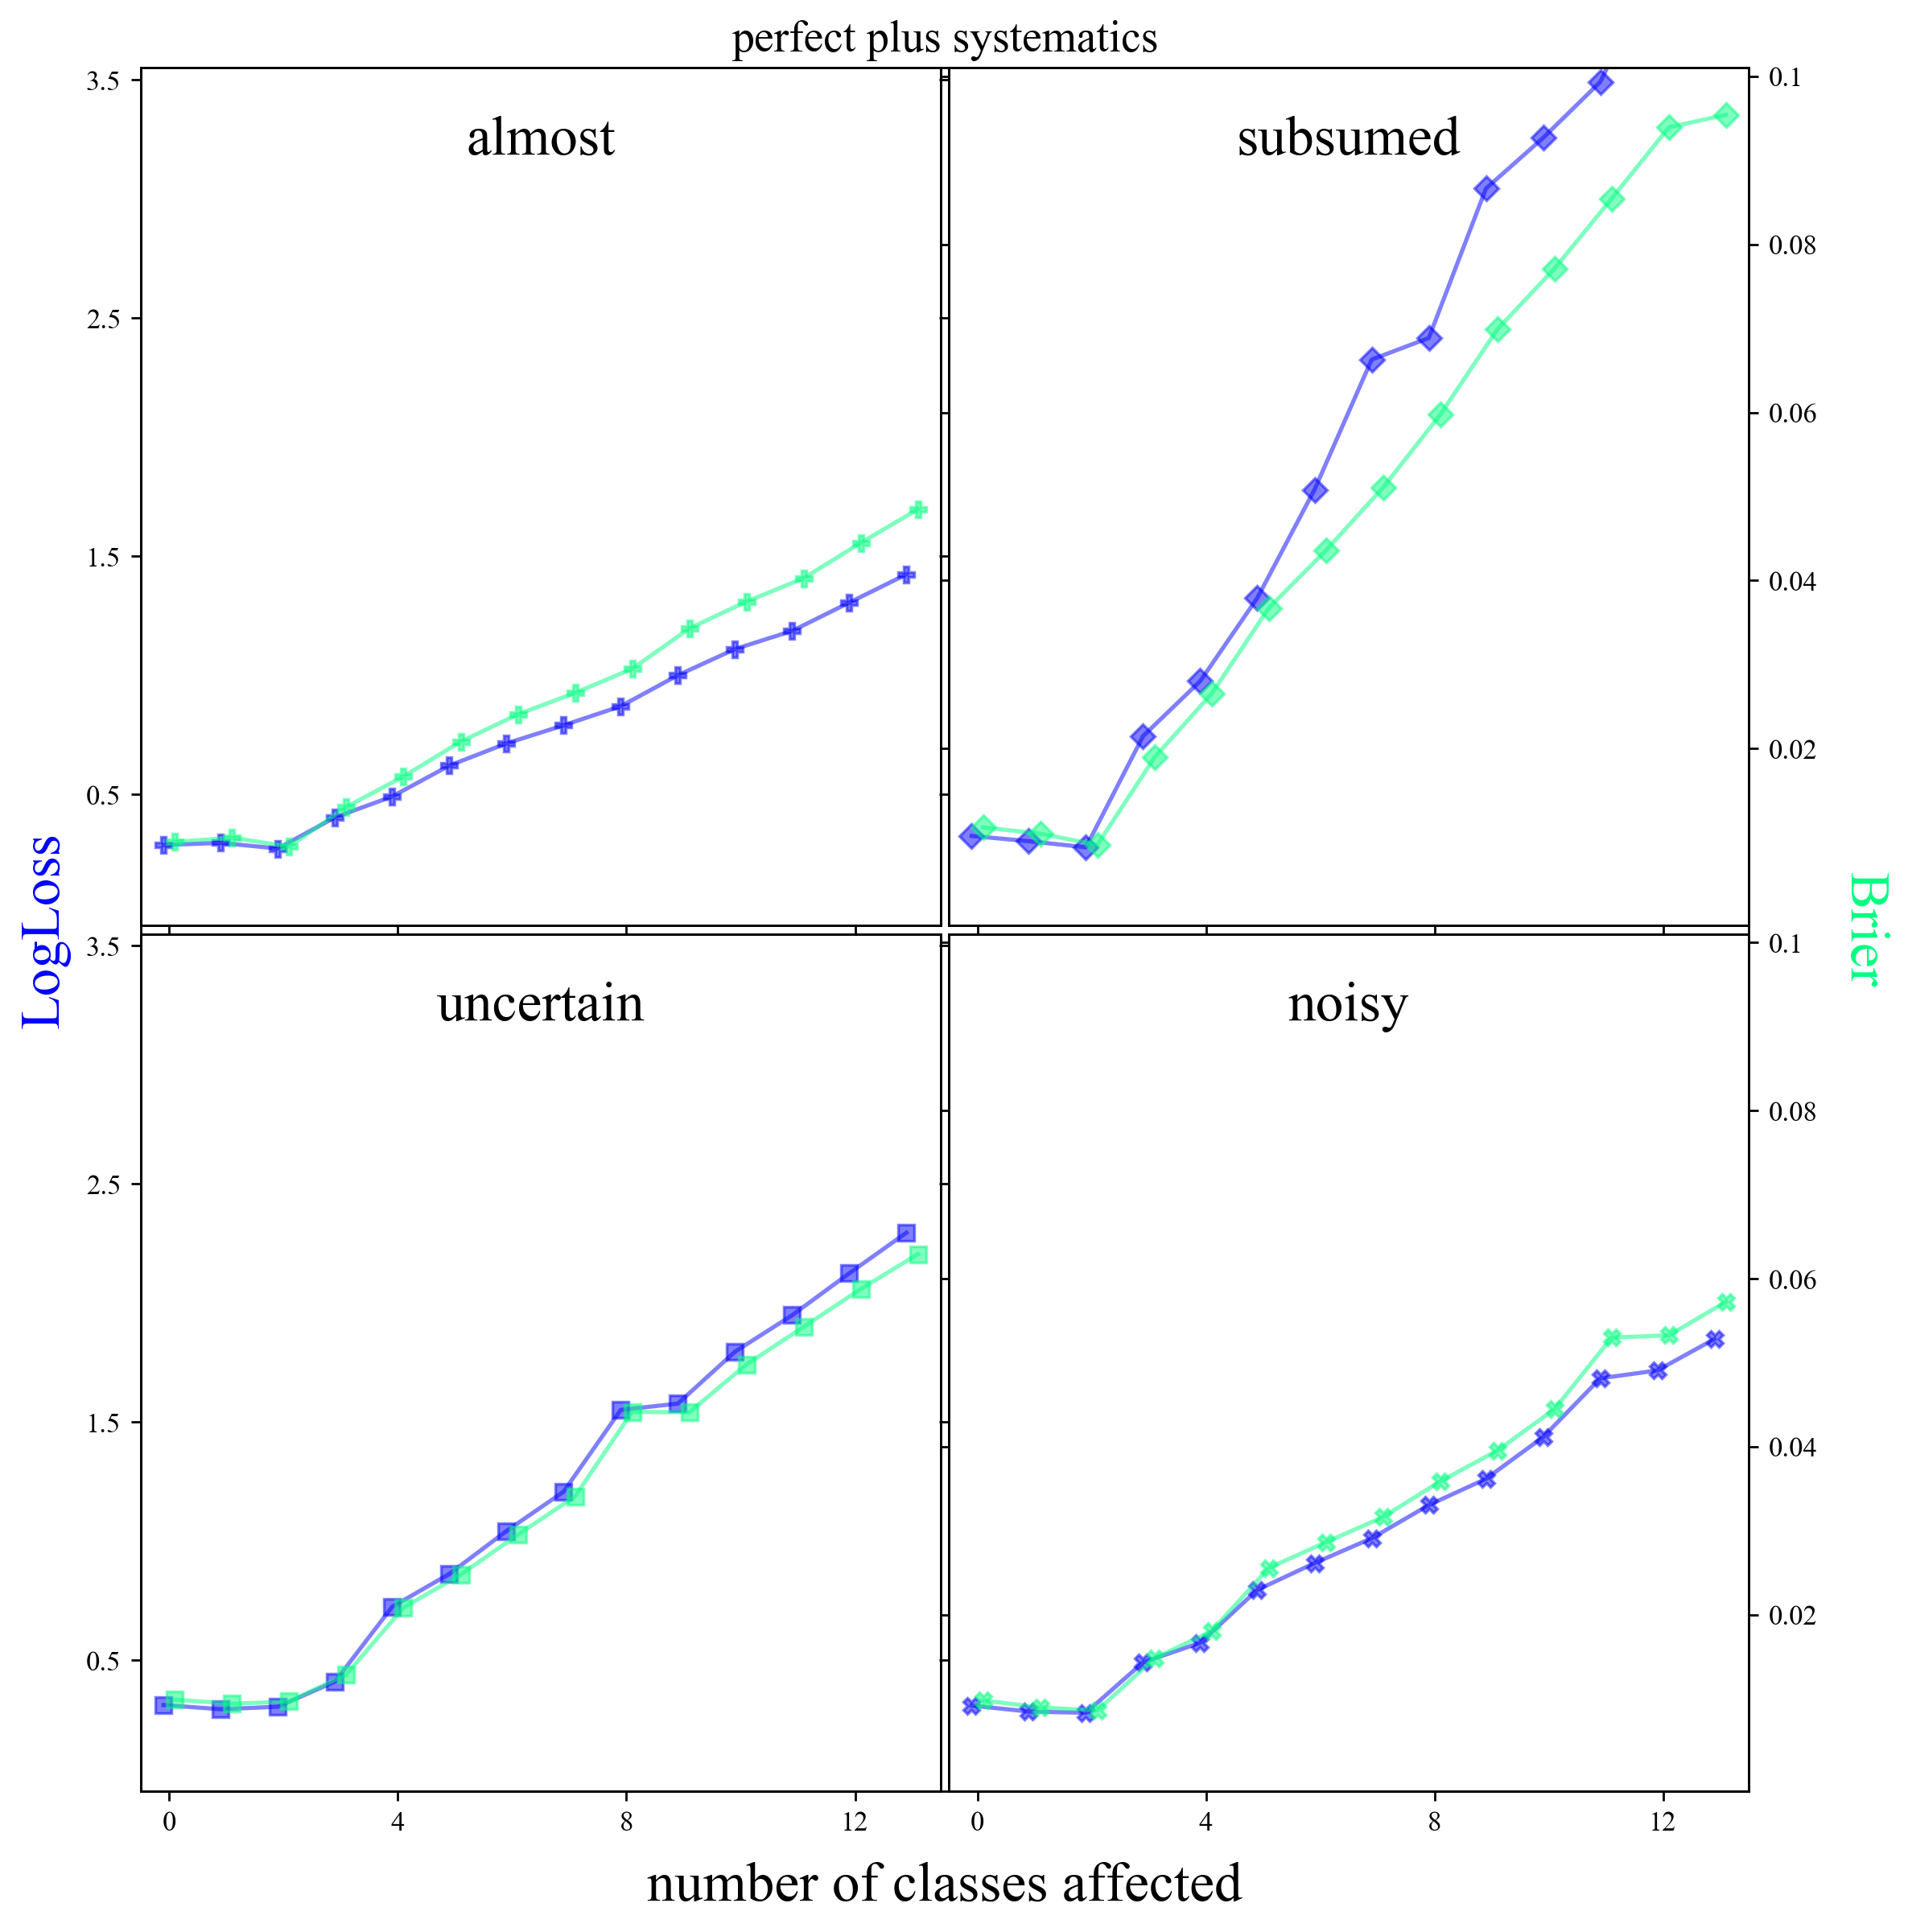
\includegraphics[width=0.5\textwidth]{./fig/systematics_onlyperfect.png}
		\caption{We confirm that the addition of systematics to the perfect classifier increases the metric values and that the increase is more or less proportional to our concerns about the systematic. \textbf{RH:green text is not visible.}}
		\label{fig:cruise}
	\end{center}
\end{figure}



\aim{Preliminary results indicate weighting will be very important for preventing the tunnel vision classifier from winning.
It may be necessary to a priori anticipate which classes will have to be most strongly protected from this systematic via upweighting them.}

\begin{figure}
	\begin{center}
		% 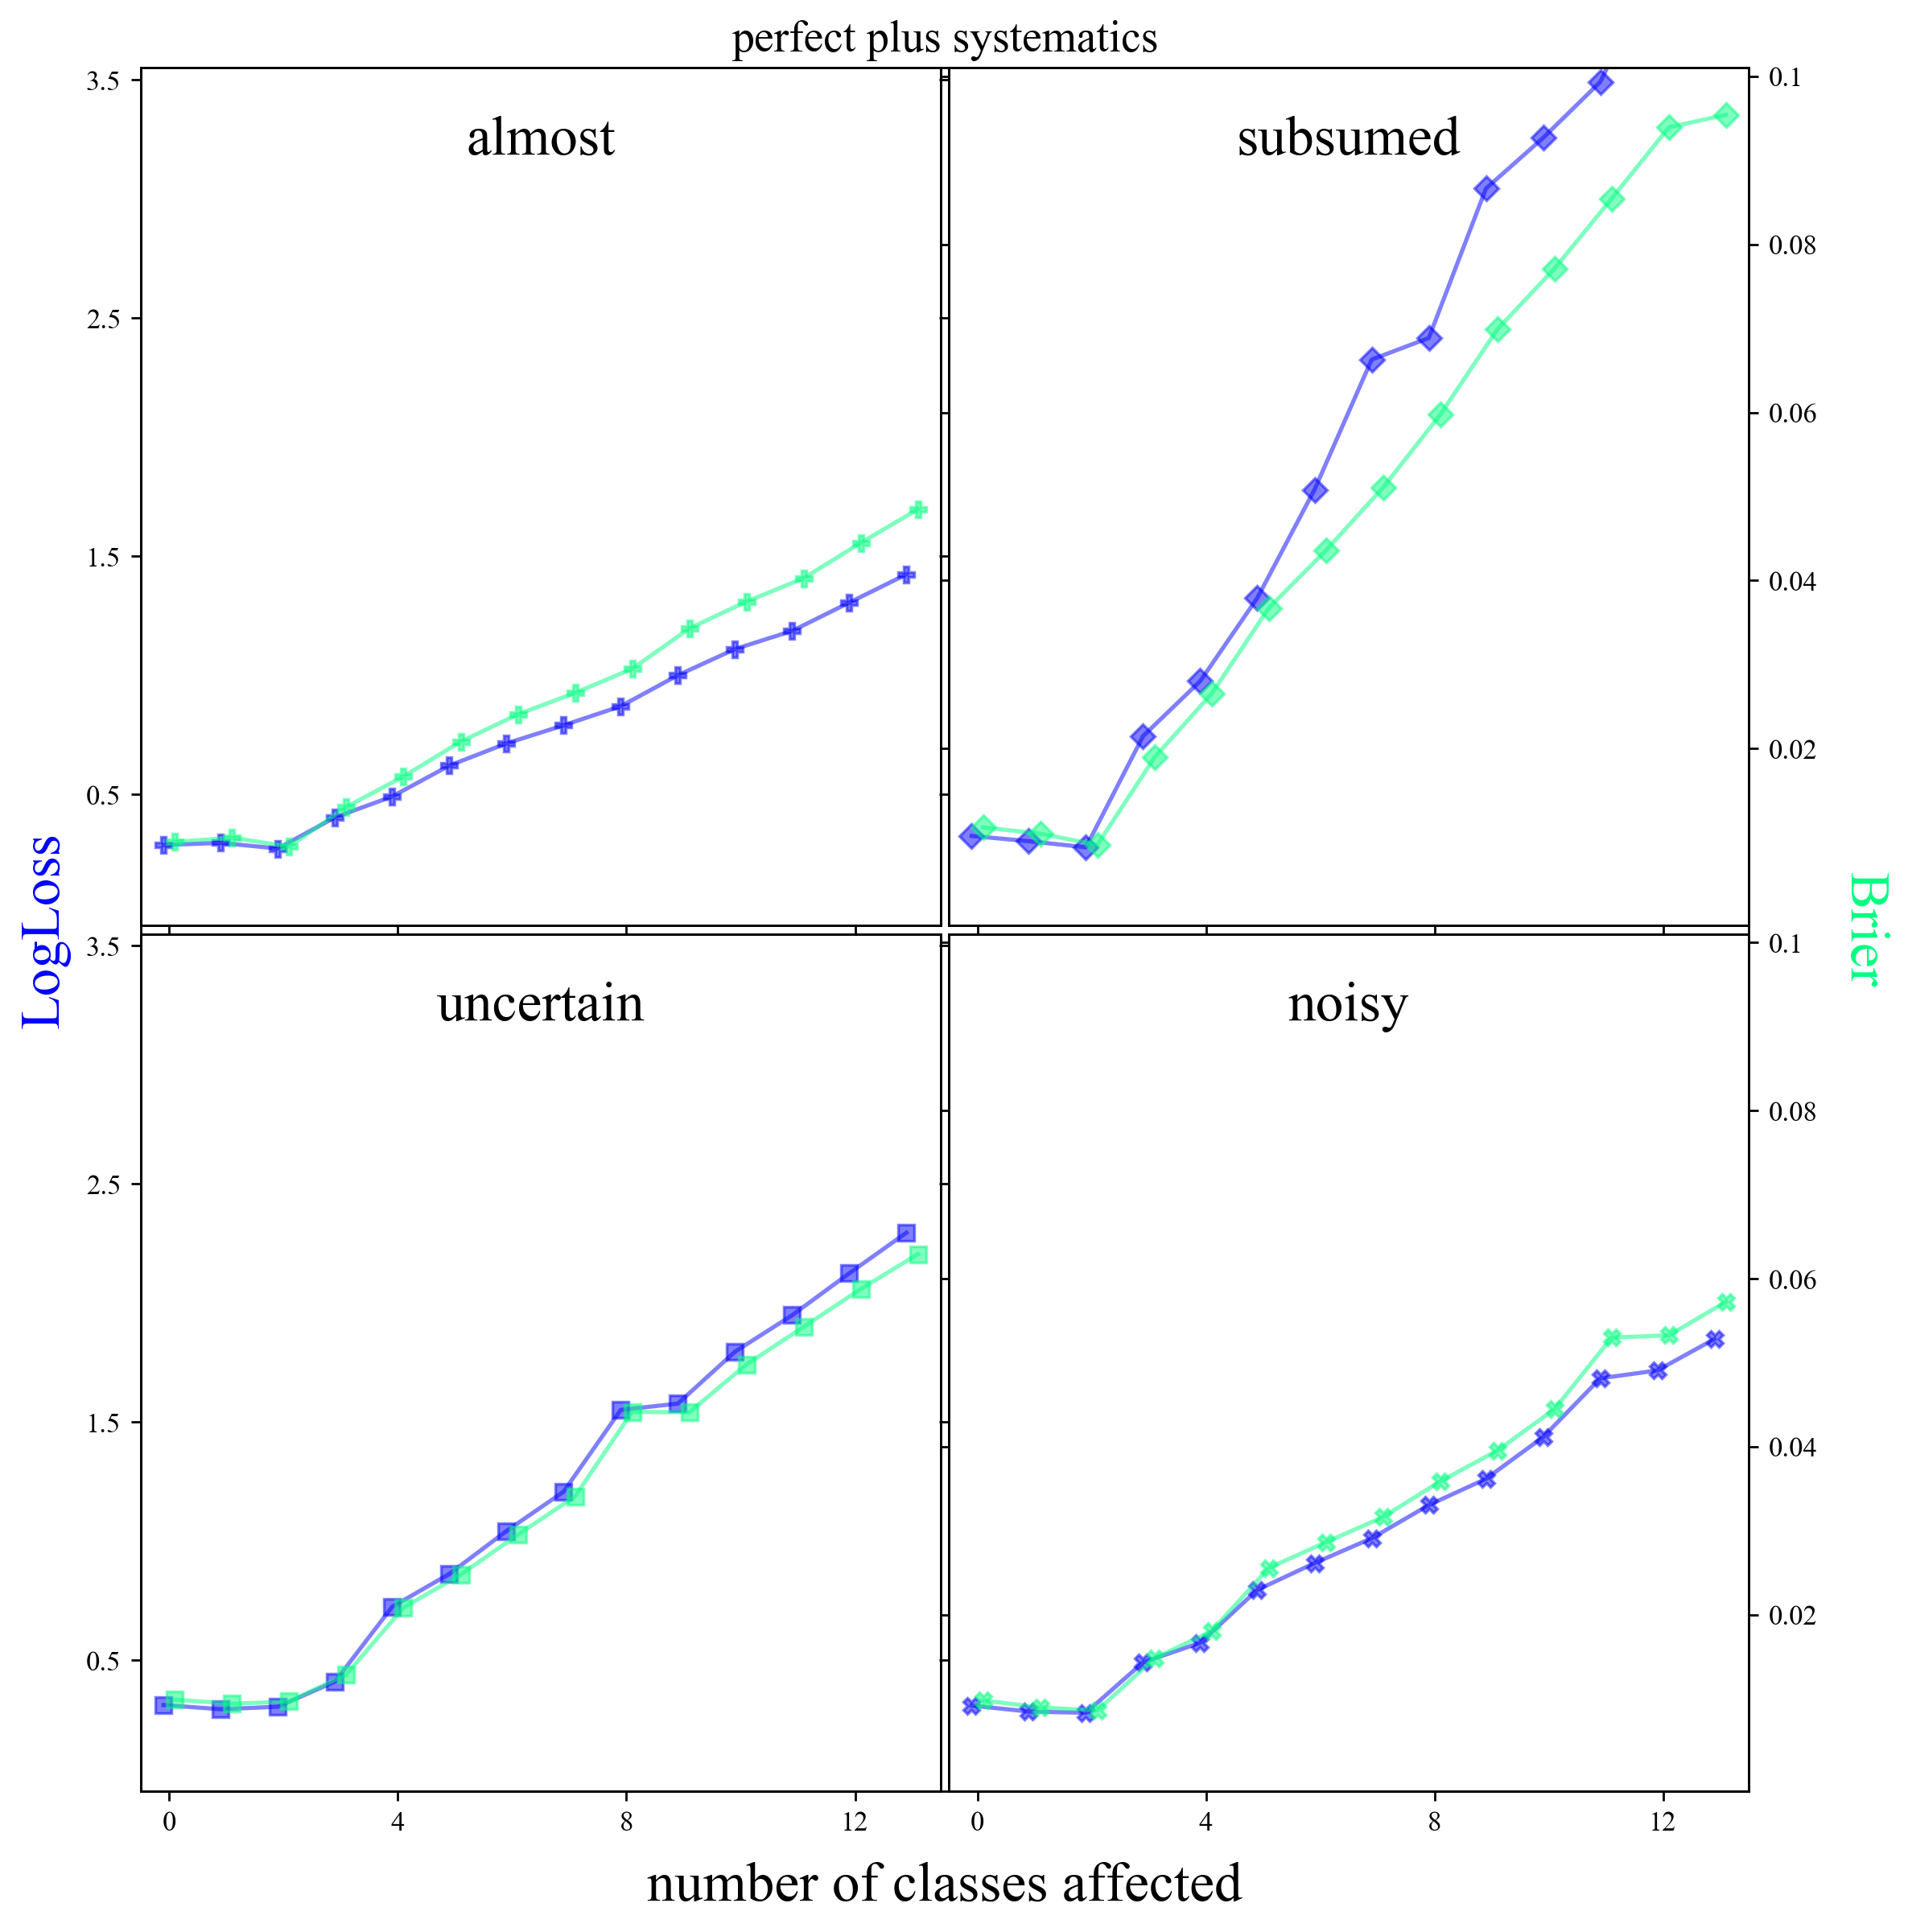
\includegraphics[width=0.5\textwidth]{./fig/systematics_onlyperfect.png}
		\caption{\aim{After much iteration on how best to present these tests, a figure similar to Figure~\ref{fig:cruise} but for the tunnel vision classifier (heading) on different baseline classifications (panels) as a function of weight on the affected class (rather than number of classes) is under construction.}}
		\label{fig:tunnel}
	\end{center}
\end{figure}

\aim{For reference, Figure~\ref{fig:popweight} shows the effect of weighting by true class population.}

\begin{figure}
	\begin{center}
		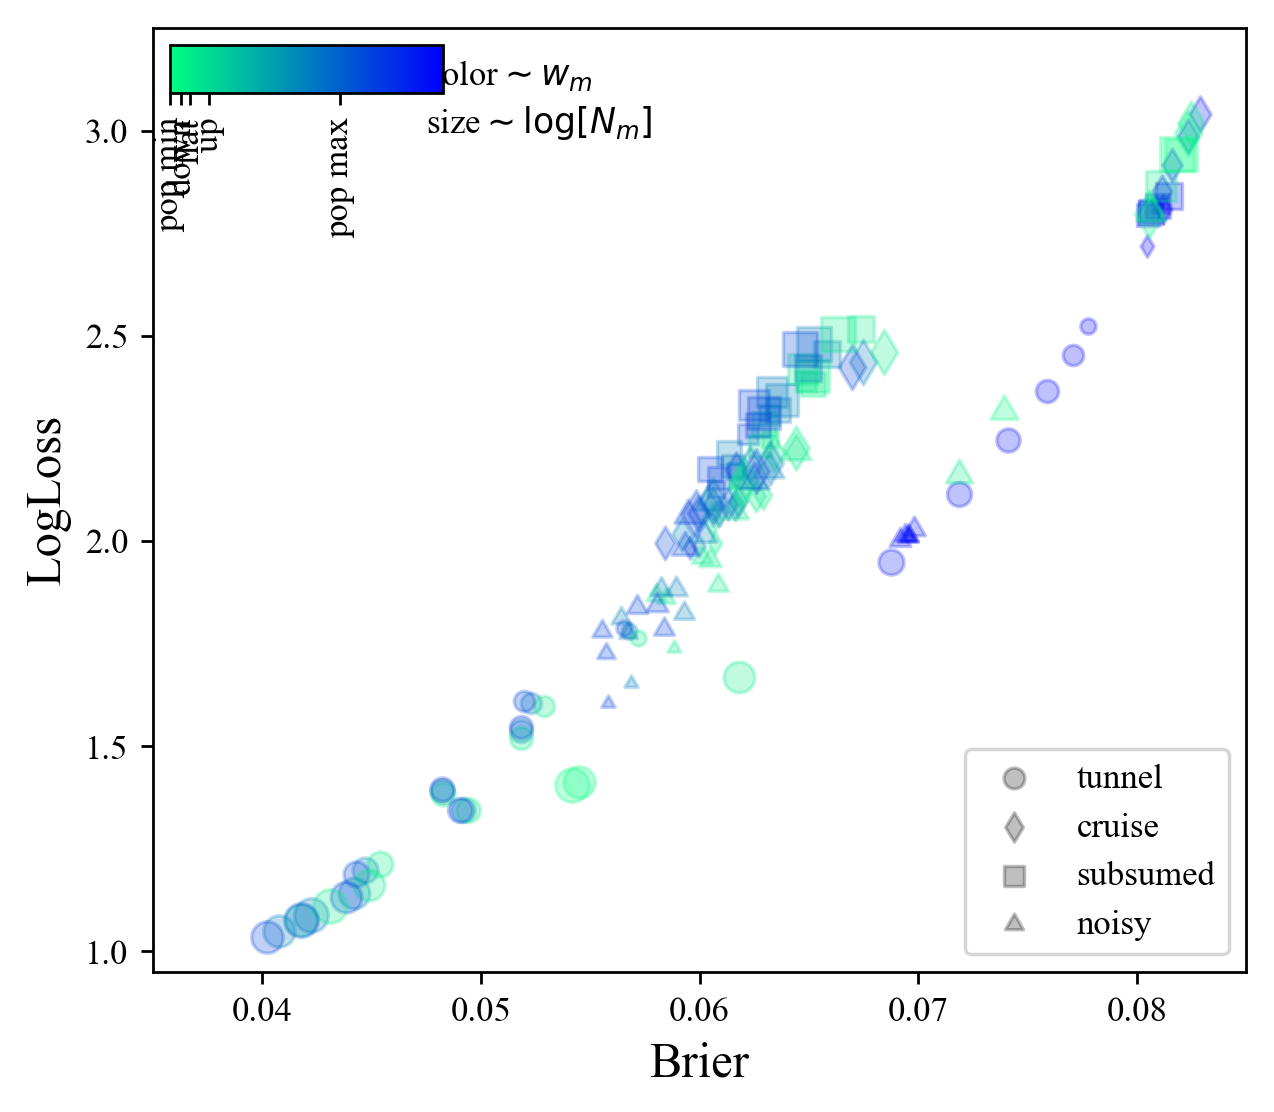
\includegraphics[width=0.5\textwidth]{./fig/all_effects_isolated.png}
		\caption{\aim{The tunnel vision classifier is hard to beat!}}
		\label{fig:popweight}
	\end{center}
\end{figure}



\subsection{Representative classifications}
\label{sec:realresults}

\begin{figure*}
	\begin{center}
		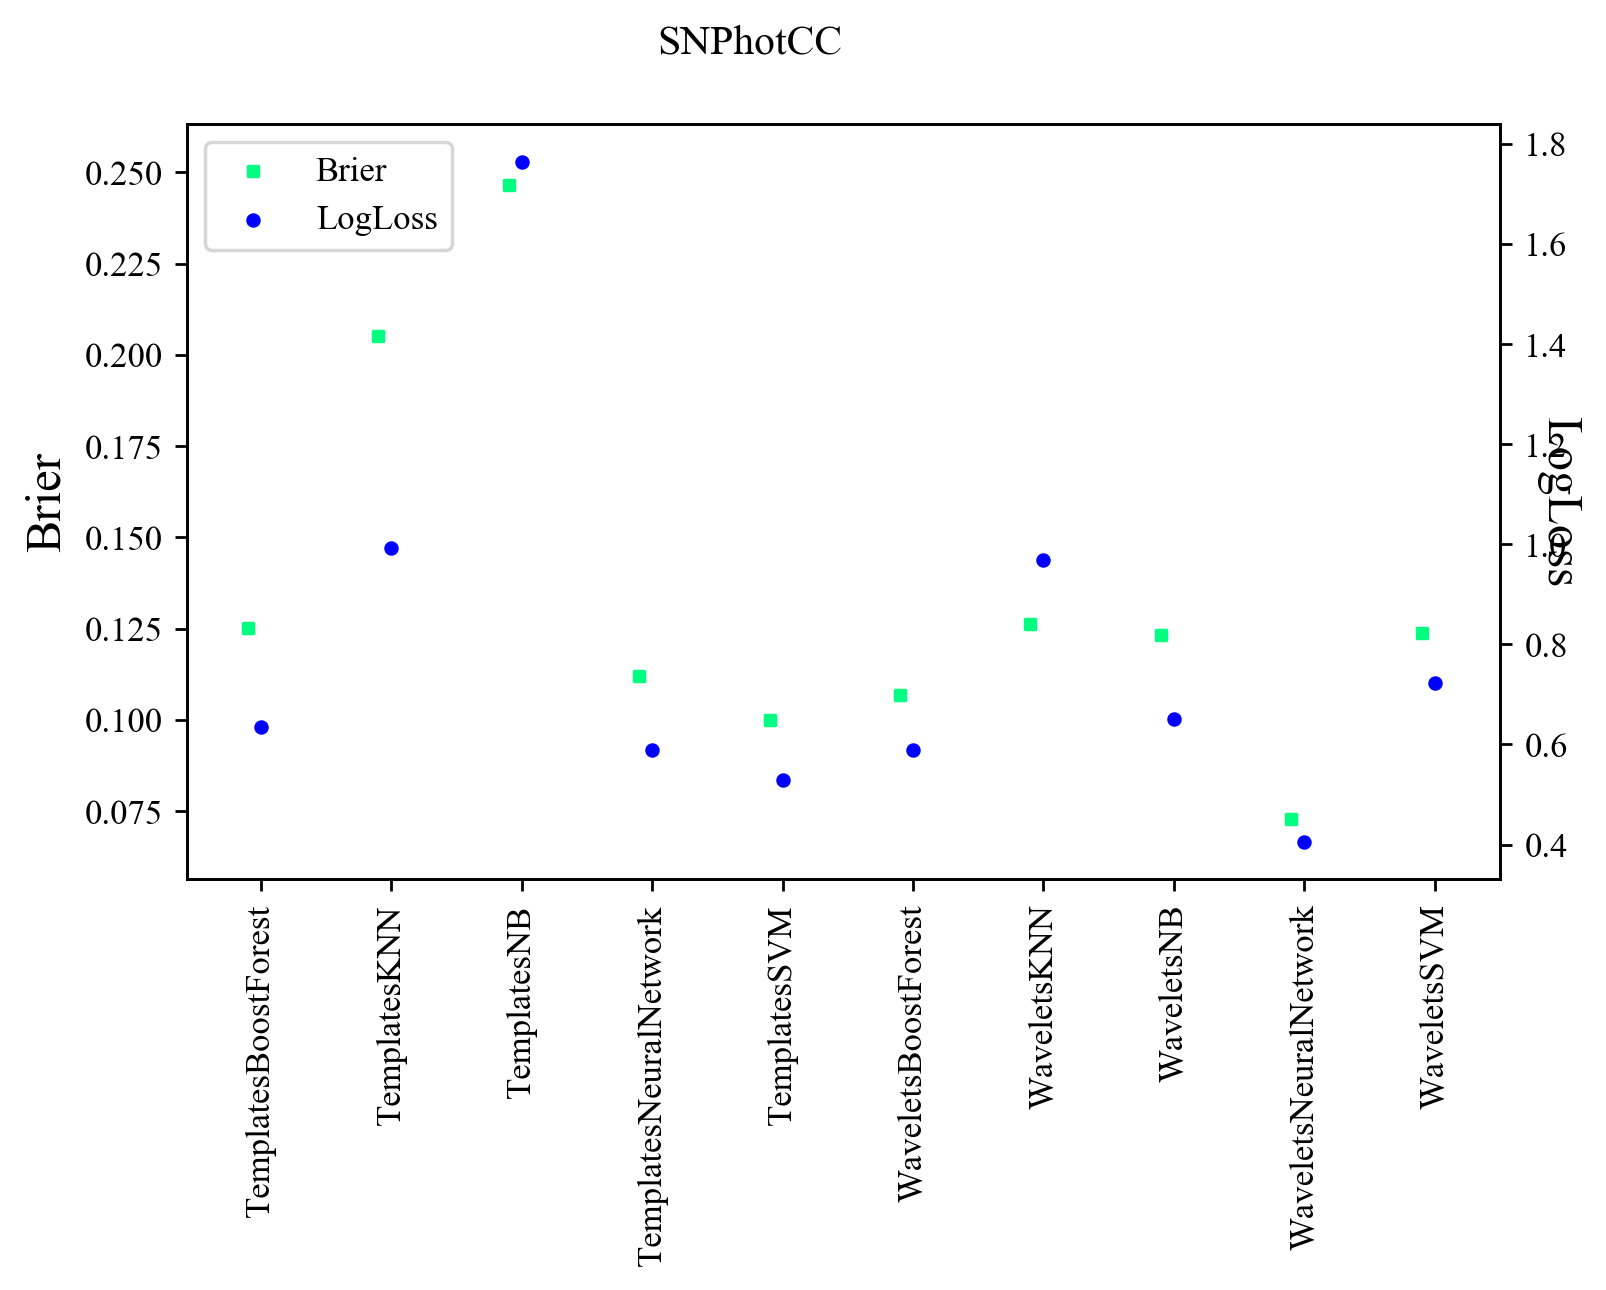
\includegraphics[width=0.45\textwidth]{./fig/SNPhotCC_res.png}
		% 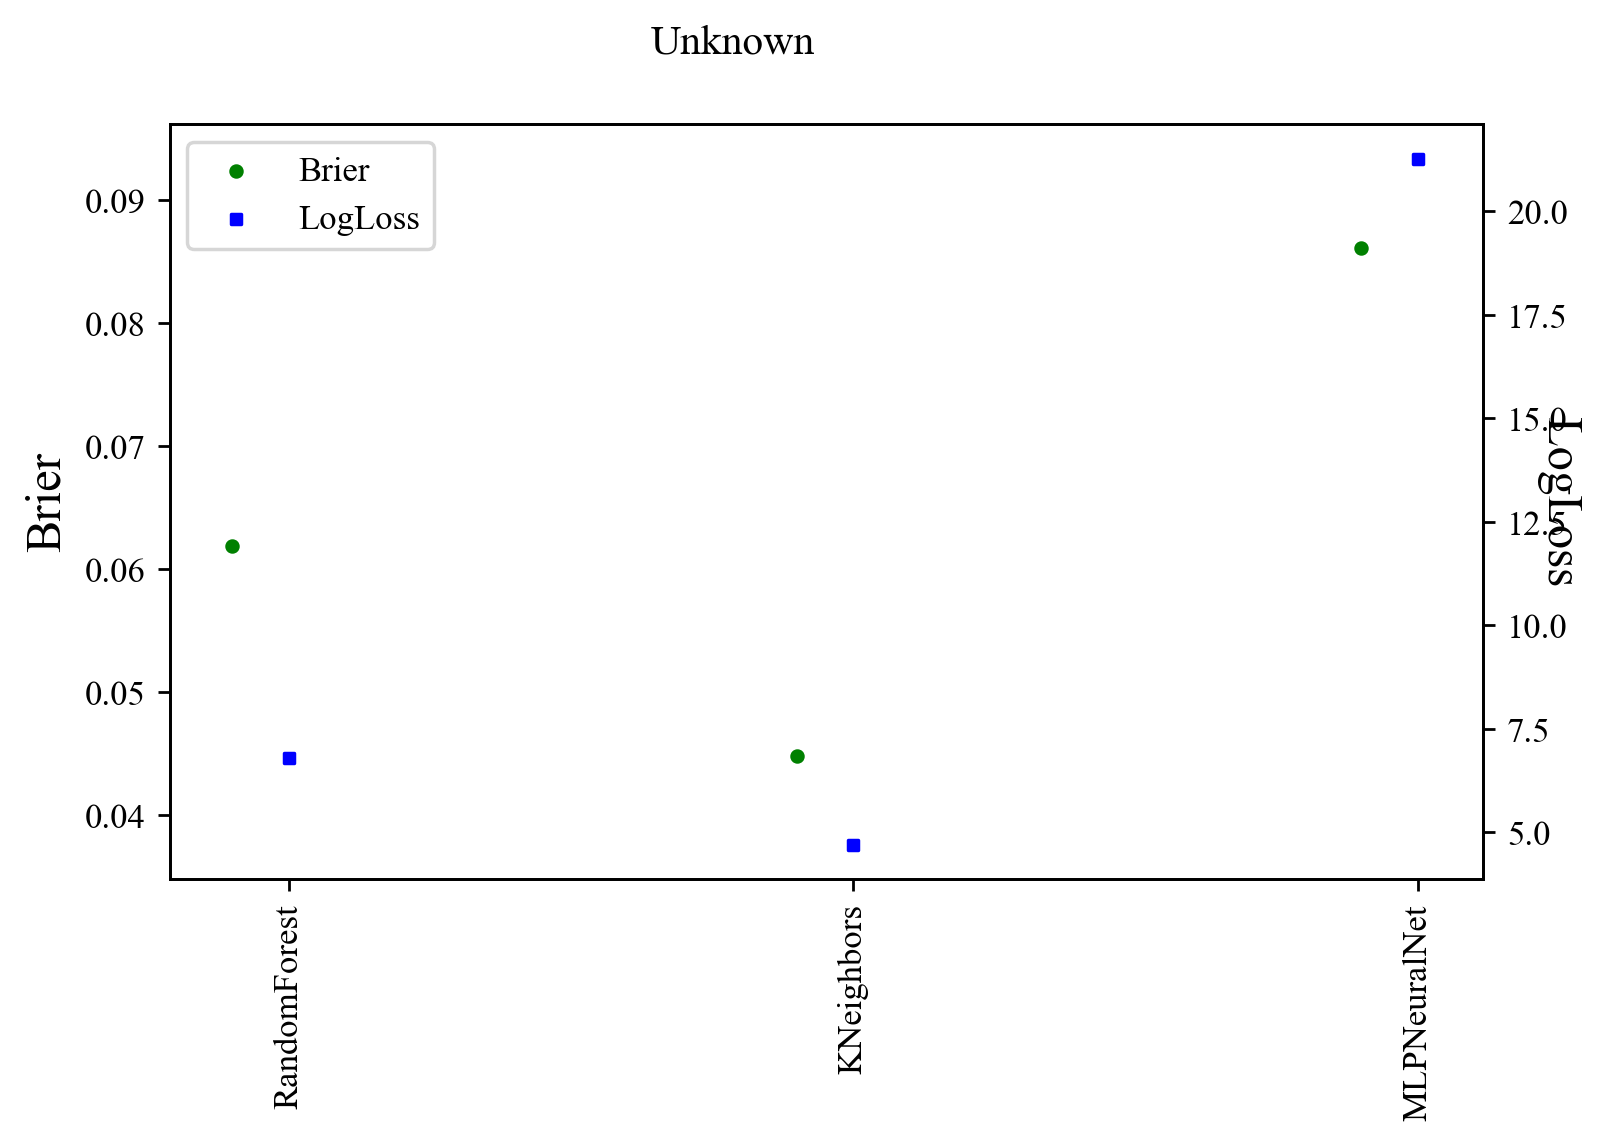
\includegraphics[width=0.45\textwidth]{./fig/Unknown_res.png}
		\caption{equal weight per class -- what kinds of weightings are meaningful to test here?  Would it be reasonable to take the real SNPhotCC entries' confusion matrices and see who would have won under each weighting/metric combination?}
		\label{fig:real_metric_compare}
	\end{center}
\end{figure*}

\textbf{We should discuss this in light of giving away too much info of the challenge - see Rick's comment.}
\aim{We are still iterating on the most informative tests to conduct on the \snphotcc\ data.
I would like to have the confusion matrices from a real classification challenge (\snphotcc\ or Ashish Mahabal's) and test different weightings of our metrics on mock classification probabilities derived from those confusion matrices to check whether we choose the same ``winner,'' but the arrangements have not yet been finalized.
The ``pipeline,'' however, is complete and ready to run as soon as the test conditions are agreed upon.}


% \subsection{Weighting systematics}
% \label{sec:weight_res}
%
% \aim{We have not yet reached consensus on what tests are reasonable in the absence of physical motivations, as the test cases here are independent of such context.}
